\chapter{Исследовательская часть}

В данном разделе будет приведен пример работы программы, а также проведен сравнительный анализ алгоритмов при различных ситуациях на основе полученных данных.

\section{Технические характеристики}

Технические характеристики устройства, на котором выполнялись замеры по времени представлены далее.

\begin{itemize}[label=---]
	\item Процессор: Intel(R) Core(TM) i5-10300H CPU 2.50 ГГц~\cite{intel}.
	\item Количество ядер: 4 физических и 8 логических ядер.
	\item Оперативная память: 16 ГБайт.
	\item Операционная система: Windows 11 Pro 64-разрядная система~\cite{windows}.
\end{itemize}

При замерах времени ноутбук был включен в сеть электропитания и был нагружен только системными приложениями.

\section{Демонстрация работы программы}

На рисунке~\ref{img:example}  представлен пример работы программы для обоих алгоритмов --- полного перебора и муравьиного. 
Осуществляется выбор файла с данными, ввод коэффициентов для муравьиного алгоритма, а также выполнение алгоритма решения задачи коммивояжера методом полного перебора и методом на основе муравьиного алгоритма.

\clearpage

\begin{figure}[h]
	\centering
	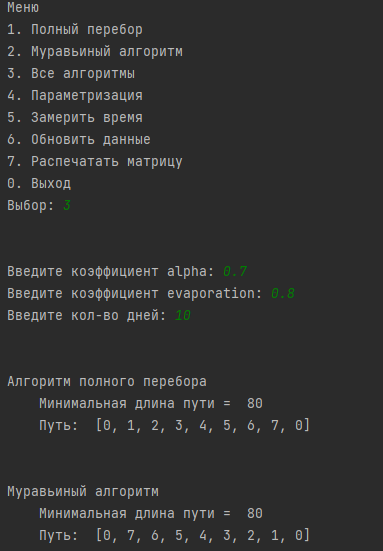
\includegraphics[width=0.5\textwidth]{img/example.png}
	\caption{Пример работы программы}
	\label{img:example}
\end{figure}

\section{Временные характеристики}

Для замера процессорного времени используется функция \\ \textit{process\_time(...)} из библиотеки \textit{time} на \textit{Python}. Функция возвращает процессорное время типа float в секундах.

Использовать функцию приходится дважды, затем из конечного времени нужно вычесть начальное, чтобы получить результат.

Замеры проводились для разного размера матриц, чтобы определить, когда наиболее эффективно использовать муравьиный алгоритм.

Результаты замеров приведены в таблице \ref{tbl:time} (время в с.).

\clearpage

\begin{table}[ht]
	\small
	\begin{center}
		\begin{threeparttable}
		\caption{Результаты замеров времени (в с.)}
		\label{tbl:time}
		\begin{tabular}{|c|c|c|}
			\hline
			\multirow{2}{*}{\bfseries Кол-во заявок} & \multicolumn{2}{c|}{\bfseries Время, мкс} \\ \cline{2-3}
			 & \bfseries Полный перебор & \bfseries Полный перебор
			\csvreader{csv/times.csv}{}
			{\\\hline \csvcoli & \csvcolii & \csvcoliii } \\
			\hline
		\end{tabular}
		\end{threeparttable}
	\end{center}
\end{table}

На рисунке~\ref{img:g1} приведен график результатов замеров времени работы реализаций алгоритмов для различных линейных размеров
матриц.

\begin{figure}[h!]
	\centering
	\begin{tikzpicture}
		\begin{axis}[	
			height = 0.4\paperheight, 
			width = 0.8\paperwidth,
			legend pos = north west,
			table/col sep=comma,
			xlabel={кол-во заявок (ед.)},
			ylabel={время, мкс},
			xmin=1.9,
			xmax=9,
			]
			\legend{ 
				Полный перебор,
				Муравьиный,
			};
			\addplot [
			solid,
			thick, 
			draw = blue,
			mark = --, 
			mark options = {
				scale = 2, 
				fill = blue, 
				draw = black
			}
			] table [x=size, y=full] {csv/times.csv};
			\addplot [
			dashed,
			thick, 
			draw = red,
			mark = --, 
			mark options = {
				scale = 2, 
				fill = blue, 
				draw = black
			}
			] table [x=size, y=ants] {csv/times.csv};
			{csv/times.csv};						
		\end{axis}
	\end{tikzpicture}
	\caption{Результаты замеров времени работы реализации конвейерной обработки}
	\label{img:g1}
\end{figure}

\clearpage

\section{Постановка эксперимента}

Автоматическая параметризация была проведена на двух классах данных --- \ref{par:class1} и \ref{par:class2}. Алгоритм будет запущен для набора значений $\alpha, \rho \in (0, 1)$.

Итоговая таблица значений параметризации будет состоять из следующих колонок:
\begin{itemize}[label=---]
	\item $\alpha$ --- коэффициент жадности;
	\item $\rho$ --- коэффициент испарения;
	\item \textit{days} --- количество дней жизни колонии муравьев;
	\item \textit{Result} --- эталонный результат, полученный методом полного перебора для проведения данного эксперимента;
	\item \textit{Mistake} --- разность полученного основанным на муравьином алгоритме методом значения и эталонного значения на данных значениях параметров, показатель качества решения.
\end{itemize}

Цель эксперимента --- определить комбинацию параметров, которые позволяют решить задачу наилучшим образом для выбранного класса данных. Качество решения зависит от количества дней и погрешности измерений.

\subsection{Класс данных 1}\label{par:class1}

Согласно с вариантом представим граф, вершины которого будут является городами путешествия за 80 дней:
\begin{enumerate}
	\item Лондон;
	\item Суэц;
	\item Бомбей;
	\item Калькутта;
	\item Гонконг;
	\item Йокогама;
	\item Сан-Франциско;
	\item Нью-Йорк.
\end{enumerate}

Занимаемый путь из:
\begin{enumerate}
	\item Лондон в Суэц за 7 дней;
	\item Суэц в Бомбей за 13 дней;
	\item Бомбей в Калькутта за 3 дня;
	\item Калькутта в Гонконг за 13 дней;
	\item Гонконг в Йокогама за 6 дней;
	\item Йокогама в Сан-Франциско за 22 дня;
	\item Сан-Франциско в Нью-Йорк за 7 дней;
	\item Нью-Йорк в Лондон за 9 дней.
\end{enumerate}

Класс данных 1 представляет собой матрицу смежности размером 8 элементов (небольшой разброс значений --- от 1 до 50), которая представлена далее.

\begin{equation}
	\label{eq:kd1}
	K_{1} = \begin{pmatrix}
		0 & 7 & 21 & 24 & 37 & 39 & 7 & 9 \\ 
		7 & 0 & 13 & 17 & 30 & 41 & 19 & 12 \\ 
		21 & 13 & 0 & 3 & 17 & 23 & 12 & 32 \\ 
		24 & 17 & 3 & 0 & 13 & 27 & 35 & 43 \\ 
		37 & 30 & 17 & 13 & 0 & 6 & 27 & 36 \\ 
		39 & 41 & 23 & 27 & 6 & 0 & 22 & 30 \\ 
		17 & 19 & 29 & 35 & 27 & 22 & 0 & 7 \\ 
		9 & 12 & 32 & 43 & 36 & 30 & 7 & 0 
	\end{pmatrix}
\end{equation}

Для данного класса данных приведена таблица \ref{tbl:table_kd1-1} -- \ref{tbl:table_kd1-3}	с выборкой параметров, которые наилучшим образом решают поставленную задачу, полные результаты параметризация приведены в приложении А. 
Использованы следующие обозначения: Days --- количество дней, Result --- результат работы, Mistake --- ошибка как отклонение решения от эталонного.

В выборке, разделенной на подгруппы по признаку значения параметра $\alpha$, для пары $(\alpha, \rho)$ выбран набор значений параметров, обеспечивающих наилучший результат приближения (наименьшее значение параметра mistake).
Если одинаковый результат параметра mistake достигается для нескольких кортежей $(\alpha, \rho, days, result, mistake)$, содержащих одинаковые значения параметров $(\alpha, \rho)$, среди них выбирается кортеж, содержащий наименьшее значение параметра days.

\begin{center}
	\captionsetup{justification=raggedright,singlelinecheck=off}
	\begin{longtable}[c]{|c|c|c|c|c|}
		\caption{Выборка из параметров для класса данных 1 (Начало)\label{tbl:table_kd1-1}}\\ \hline
		$\alpha$ & $\rho$ & Days & Result & Mistake \\ \hline
		0.1 & 0.1 &  1 &   80 &    0 \\
		0.1 & 0.2 &  5 &   80 &    0 \\
		0.1 & 0.3 &  5 &   80 &    0 \\
		0.1 & 0.4 &  10 &   80 &    0 \\
		0.1 & 0.5 &  5 &   80 &    0 \\
		0.1 & 0.6 &  50 &   80 &    0 \\
		0.1 & 0.7 &  50 &   80 &    0 \\
		0.1 & 0.8 &  5 &    80 &    0 \\ \hline
		0.2 & 0.1 &  10 &   80 &    0 \\
		0.2 & 0.2 &  50 &   80 &    0 \\
		0.2 & 0.3 &  10 &   80 &    0 \\
		0.2 & 0.4 &  10 &   80 &    0 \\
		0.2 & 0.5 &  50 &   80 &    0 \\
		0.2 & 0.6 &  50 &   80 &    0 \\
		0.2 & 0.7 &  10 &   80 &    0 \\
		0.2 & 0.8 &  50 &  80 &    0 \\ \hline
		0.3 & 0.1 &  10 &   80 &    0 \\
		0.3 & 0.2 &  100 &   80 &    0 \\
		0.3 & 0.3 &  50 &   80 &    0 \\
		0.3 & 0.4 &  10 &   80 &    0 \\ \hline
	\end{longtable}
\end{center}

\clearpage

\begin{center}
	\captionsetup{justification=raggedright,singlelinecheck=off}
	\begin{longtable}[c]{|c|c|c|c|c|}
		\caption{Выборка из параметров для класса данных 1 (Продолжение)\label{tbl:table_kd1-2}}\\ \hline
		$\alpha$ & $\rho$ & Days & Result & Mistake \\ \hline
		0.3 & 0.5 &  100 &   80 &    0 \\
		0.3 & 0.6 &  50 &   80 &    0 \\
		0.3 & 0.7 &  100 &   80 &    0 \\
		0.3 & 0.8 &  50 &  80 &    0 \\ \hline
		0.4 & 0.1 &  50 &   80 &    0 \\
		0.4 & 0.2 &  50 &   80 &    0 \\
		0.4 & 0.3 &  50 &   80 &    0 \\
		0.4 & 0.4 &  10 &   80 &    0 \\
		0.4 & 0.5 &  50 &   80 &    0 \\
		0.4 & 0.6 &  50 &   80 &    0 \\
		0.4 & 0.7 &  50 &   80 &    0 \\	
		0.4 & 0.8 &  50 &  80 &    0 \\ \hline
		0.5 & 0.1 &  50 &   80 &    0 \\
		0.5 & 0.2 &  50 &   80 &    0 \\
		0.5 & 0.3 &  50 &   80 &    0 \\
		0.5 & 0.4 &  10 &   80 &    0 \\
		0.5 & 0.5 &  50 &   80 &    0 \\
		0.5 & 0.6 &  100 &   80 &    0 \\
		0.5 & 0.7 &  50 &   80 &    0 \\
		0.5 & 0.8 &  300 &  80 &    0 \\ \hline
		0.6 & 0.1 & 100 &   80 &    0 \\
		0.6 & 0.2 & 50 &   80 &    0 \\
		0.6 & 0.3 & 100 &   80 &    0 \\
		0.6 & 0.4 & 100 &   80 &    0 \\
		0.6 & 0.5 & 50 &   80 &    0 \\
		0.6 & 0.6 & 50 &   80 &    0 \\
		0.6 & 0.7 & 10 &   80 &    0 \\
		0.6 & 0.8 & 100 &  80 &    0 \\ \hline
		0.7 & 0.1 & 100 &   80 &    0 \\
		0.7 & 0.2 & 50 &   80 &    0 \\ \hline
	\end{longtable}
\end{center}

\begin{center}
	\captionsetup{justification=raggedright,singlelinecheck=off}
	\begin{longtable}[c]{|c|c|c|c|c|}
		\caption{Выборка из параметров для класса данных 1 (Продолжение)\label{tbl:table_kd1-3}}\\ \hline
		$\alpha$ & $\rho$ & Days & Result & Mistake \\ \hline
		0.7 & 0.3 & 50 &   80 &    0 \\
		0.7 & 0.4 & 100 &   80 &    0 \\
		0.7 & 0.5 & 50 &   80 &    0 \\
		0.7 & 0.6 & 50 &   80 &    0 \\
		0.7 & 0.7 & 10 &   80 &    0 \\
		0.8 & 0.8 & 10 &  80 &    0 \\ \hline
		0.8 & 0.1 & 50 &   80 &    0 \\
		0.8 & 0.2 & 300 &   80 &    0 \\
		0.8 & 0.3 & 100 &   80 &    0 \\
		0.8 & 0.4 & 300 &   80 &    0 \\
		0.8 & 0.5 & 300 &   80 &    0 \\
		0.8 & 0.6 & 100 &   80 &    0 \\
		0.8 & 0.7 & 300 &   80 &    0 \\
		0.8 & 0.8 & 50 &  80 &    0 \\ \hline
		0.9 & 0.1 & 300 &   80 &    0 \\
		0.9 & 0.2 & 300 &   80 &    0 \\
		0.9 & 0.3 & 100 &   80 &    0 \\
		0.9 & 0.4 & 80 &   80 &    0 \\
		0.9 & 0.5 & 300 &   80 &    0 \\
		0.9 & 0.6 & 50 &   80 &    0 \\
		0.9 & 0.7 & 100 &   80 &    0 \\
		0.9 & 0.8 & 50 &  80 &    0 \\ \hline
	\end{longtable}
\end{center}

\clearpage

\subsection{Класс данных 2}\label{par:class2}

Класс данных 2 представляет собой матрицу смежности размером 9 элементов (большой разброс значений - от 1000 до 9999), которая представлена далее.

\begin{equation}
	\label{eq:kd2}
	K_{1} = \begin{pmatrix}
		0 & 1470 & 6489 & 2010 & 9573 & 2842 & 4881 & 5450 \\
		1470 & 0 & 3721 & 9794 & 4278 & 6202 & 3552 & 1825 \\
		1825 & 3721 & 0 & 6856 & 6856 & 8202 & 7770 & 9909 \\
		4924 & 9794 & 6856 & 0 & 4036 & 3150 & 8496 & 5701 \\
		9573 & 4278 & 1177 & 4036 & 0 & 4467 & 3438 & 4887 \\
		2842 & 6202 & 8202 & 3150 & 4467 & 0 & 6736 & 3139 \\
		4881 & 3552 & 7770 & 8496 & 3438 & 6736 & 0 & 3716 \\
		5450 & 1825 & 9909 & 5701 & 4887 & 3139 & 3716 & 0 \\
	\end{pmatrix}
\end{equation}

Для данного класса данных приведена таблица \ref{tbl:table_kd2-1} -- \ref{tbl:table_kd2-3}	с выборкой параметров, которые наилучшим образом решают поставленную задачу, полные результаты параметризация приведены в приложении Б. 

\clearpage

\begin{center}
	\captionsetup{justification=raggedright,singlelinecheck=off}
	\begin{longtable}[c]{|c|c|c|c|c|}
		\caption{Выборка из параметров для класса данных 2 (Начало)\label{tbl:table_kd2-1}}\\ \hline
		$\alpha$ & $\rho$ & Days & Result & Mistake \\ \hline
		0.1 & 0.1 &  50 &   24474 &    0 \\
		0.1 & 0.2 &  3 &   24474 &    0 \\
		0.1 & 0.3 &  3 &   24474 &    0 \\
		0.1 & 0.4 &  1 &   24474 &    0 \\
		0.1 & 0.5 &  10 &   24474 &    0 \\
		0.1 & 0.6 &  50 &   24474 &    0 \\
		0.1 & 0.7 &  100 &   24474 &    0 \\
		0.1 & 0.8 &  50 &    24474 &    0 \\ \hline
		0.2 & 0.1 &  10 &   24474 &    0 \\
		0.2 & 0.2 &  5 &   24474 &    0 \\
		0.2 & 0.3 &  50 &   24474 &    0 \\
		0.2 & 0.4 &  10 &   24474 &    0 \\
		0.2 & 0.5 &  3 &   24474 &    0 \\
		0.2 & 0.6 &  50 &   24474 &    0 \\
		0.2 & 0.7 &  50 &   24474 &    0 \\
		0.2 & 0.8 &  10 &  24474 &    0 \\ \hline
		0.3 & 0.1 &  10 &   24474 &    0 \\
		0.3 & 0.2 &  100 &   24474 &    0 \\
		0.3 & 0.3 &  5 &   24474 &    0 \\
		0.3 & 0.4 &  10 &   24474 &    0 \\
		0.3 & 0.5 &  100 &   24474 &    0 \\
		0.3 & 0.6 &  50 &   24474 &    0 \\
		0.3 & 0.7 &  100 &   24474 &    0 \\
		0.3 & 0.8 &  50 &  24474 &    0 \\ \hline
		0.4 & 0.1 &  50 &   24474 &    0 \\
		0.4 & 0.2 &  100 &   24474 &    0 \\
		0.4 & 0.3 &  50 &   24474 &    0 \\
		0.4 & 0.4 &  50 &   24474 &    0 \\
		0.4 & 0.5 &  100 &   24474 &    0 \\ \hline
	\end{longtable}
\end{center}

\clearpage

\begin{center}
	\captionsetup{justification=raggedright,singlelinecheck=off}
	\begin{longtable}[c]{|c|c|c|c|c|}
		\caption{Выборка из параметров для класса данных 2 (Продолжение)\label{tbl:table_kd2-2}}\\ \hline
		$\alpha$ & $\rho$ & Days & Result & Mistake \\ \hline
		0.4 & 0.6 &  50 &   24474 &    0 \\
		0.4 & 0.7 &  10 &   24474 &    0 \\	
		0.4 & 0.8 &  50 &  24474 &    0 \\ \hline
		0.5 & 0.1 &  300 &   24474 &    0 \\
		0.5 & 0.2 &  100 &   24474 &    0 \\
		0.5 & 0.3 &  50 &   24474 &    0 \\
		0.5 & 0.4 &  300 &   24474 &    0 \\
		0.5 & 0.5 &  300 &   24474 &    0 \\
		0.5 & 0.6 &  300 &   24474 &    0 \\
		0.5 & 0.7 &  50 &   24474 &    0 \\
		0.5 & 0.8 &  300 &  24474 &    0 \\ \hline
		0.6 & 0.1 & 50 &   24474 &    0 \\
		0.6 & 0.2 & 100 &   24474 &    0 \\
		0.6 & 0.3 & 100 &   24474 &    0 \\
		0.6 & 0.4 & 300 &   24474 &    0 \\
		0.6 & 0.5 & 50 &   24474 &    0 \\
		0.6 & 0.6 & 300 &   24474 &    0 \\
		0.6 & 0.7 & 10 &   24474 &    0 \\
		0.6 & 0.8 & 50 &  24474 &    0 \\ \hline
		0.7 & 0.1 & 100 &   24474 &    0 \\
		0.7 & 0.2 & 100 &   24474 &    0 \\
		0.7 & 0.3 & 50 &   24474 &    0 \\
		0.7 & 0.4 & 50 &   24474 &    0 \\
		0.7 & 0.5 & 50 &   24474 &    0 \\
		0.7 & 0.6 & 100 &   24474 &    0 \\
		0.7 & 0.7 & 300 &   24474 &    0 \\
		0.8 & 0.8 & 300 &  24474 &    0 \\ \hline
		0.8 & 0.1 & 50 &   24474 &    0 \\
		0.8 & 0.2 & 50 &   24474 &    0 \\ \hline
		
	\end{longtable}
\end{center}

\begin{center}
	\captionsetup{justification=raggedright,singlelinecheck=off}
	\begin{longtable}[c]{|c|c|c|c|c|}
		\caption{Выборка из параметров для класса данных 2 (Продолжение)\label{tbl:table_kd2-3}}\\ \hline
		$\alpha$ & $\rho$ & Days & Result & Mistake \\ \hline
		0.8 & 0.3 & 100 &   24474 &    0 \\
		0.8 & 0.4 & 100 &   24474 &    0 \\
		0.8 & 0.5 & 10 &   24474 &    0 \\
		0.8 & 0.6 & 50 &   24474 &    0 \\
		0.8 & 0.7 & 300 &   24474 &    0 \\
		0.8 & 0.8 & 50 &  24474 &    0 \\ \hline
		0.9 & 0.1 & 100 &   24474 &    0 \\
		0.9 & 0.2 & 300 &   24474 &    0 \\
		0.9 & 0.3 & 300 &   24474 &    0 \\
		0.9 & 0.4 & 100 &   24474 &    0 \\
		0.9 & 0.5 & 100 &   24474 &    0 \\
		0.9 & 0.6 & 100 &   24474 &    0 \\
		0.9 & 0.7 & 100 &   24474 &    0 \\
		0.9 & 0.8 & 300 &  24474 &    0 \\ \hline
	\end{longtable}
\end{center}

\section{Вывод}

В результате эксперимента было получено, что использование муравьиного алгоритма наиболее эффективно при больших размерах матриц. Так, при размере матрицы, равном 2, муравьиный алгоритм меленее алгоритма полного перебора в 143 раза, а при размере матрицы, равном 9, муравьиный алгоритм быстрее алгоритма полного перебора в раз, а при размере в 10 -- уже в 15 раз. Следовательно, при размерах матриц больше 8 следует использовать муравьиный алгоритм, но стоит учитывать, что он не гарантирует получения глобального оптимума при решении задачи.

Также при проведении эксперимента с классами данных было получено, что на первом классе данных (см. п. \ref{par:class1}) муравьиный алгоритм лучше всего показывает себя при параметрах:
\begin{itemize}[label=---]
	\item $\alpha = 0.1, \rho = 0.1, days = 1$;
	\item $\alpha = 0.2, \rho \in \{0.1, 0.3, 0.4, 0.7\}, days = 10$;
	\item $\alpha = 0.3, \rho \in \{0.1, 0.4\}, days = 10$;
	\item $\alpha = 0.4, \rho = 0.4, days = 10$;
	\item $\alpha = 0.5, \rho = 0.4, days = 10$;
	\item $\alpha = 0.6, \rho = 0.7, days = 10$;
	\item $\alpha = 0.7, \rho \in \{0.7, 0.8\}, days = 10$.
\end{itemize}  

Следовательно, для класса данных 1 рекомендуется использовать данные параметры. 

Для класса данных 2 (см. п. \ref{par:class2}) было получено, что наилучшим образом алгоритм работает на значениях параметров, которые представлены далее:
\begin{itemize}[label=---]
	\item $\alpha = 0.1, \rho = 0.4, days = 1$;
	\item $\alpha = 0.2, \rho = 0.5, days = 3$;
	\item $\alpha = 0.3, \rho = 0.3, days = 5$;
	\item $\alpha = 0.4, \rho = 0.7, days = 10$;
	\item $\alpha = 0.6, \rho = 0.7, days = 10$;
	\item $\alpha = 0.8, \rho = 0.5, days = 10$.
\end{itemize} 

Для второго класса данных 2 рекомендуется использовать данные параметры.
